\documentclass[letterpaper,11pt]{article}
\usepackage{science}
\usepackage[utf8]{inputenc}
\usepackage{mathtools}
\usepackage{subcaption}
\usepackage{tikz}
\usepackage{pgf}
\usepackage{pgfplots}
\usepackage{circuitikz}
\usepackage{tabularx}
\usepackage{array}
\usepackage{booktabs} 
\usepackage{colortbl} 
\usepackage{xfrac}
\usepackage{gensymb}

\usetikzlibrary{calc}

\title{\textbf{Ottica:} esperienza 4}
\author{Canteri Marco, Biasi Lorenzo, Damiani Emily}
\date{\today}

\begin{document}
\maketitle

\begin{abstract}
\hspace{-1.9em}
Scopo dell'esperienza è la misura dell'indice di rifrazione di 4 materiali diversi in funzione della lunghezza d'onda della luce. 
\end{abstract}

\begin{body}
\section{Procedimento}
Per la misura dell'indice di rifrazione abbiamo utilizzato 4 prismi di materiale diverso: 
\begin{itemize}
\item acqua 
\item plexiglas
\item vetro standard
\item vetro F 
\end{itemize}
e di una lampada all'elio di cui conosciamo lo spettro, quindi il valore delle lunghezze d'onda dei picchi massimi di intensità. Il prisma è stato posizionato sulla piattaforma rotante davanti alla lampada e dietro di esso si trova il foto-detector che mostra a schermo il grafico ($\theta$, Intensità luminosa). In questo esperimento la posizione del prisma sulla piattaforma è fondamentale. Sappiamo infatti, che il raggio di luce incidente sul prisma viene deviato secondo un angolo che dipende dall'indice di rifrazione del materiale e che l'angolo di uscita dipende dall'angolo di incidenza del raggio luminoso. Data la geometria del prisma, l'angolo di deviazione minima si ottiene puntando il raggio parallelamente alla sua base, ed è proprio quest'angolo che andremo a misurare. Per posizionare il prisma nel modo opportuno si  muove la piattaforma cercando il punto in cui il raggio luminoso rifratto dal prisma si muove in avanti e poi torna indietro. \\
Una volta sistemato il prisma si posiziona l'angolo di partenza a $0$ e si procede con la scansione dell'intensità muovendo il fotodetector. \\
Per ogni materiale si sono effettuate le misure 4 volte in modo tale da riconoscere meglio i picchi dal rumore di fondo e il valore di angolo corrispondente. Una volta ottenuto il grafico, questo andrà confrontato con lo spettro dell'elio in funzione della lunghezza d'onda, in modo tale da associare ad un angolo $\theta_{min}$ un unico valore di lunghezza d'onda $\lambda$. Confrontare i due grafici può non essere facile, a causa dei limiti nell'apparecchiatura stessa. Per questo motivo può essere utile eseguire la scansione di un raggio laser, di cui si conosce la lunghezza d'onda ($650 nm)$ e sapere approssimativamente a quale angolo è associato, per orientarsi meglio nel confronto. Inoltre per mettere a fuoco bene il raggio rifratto sul sensore può essere utile munirsi di due lenti, poste tra la lampada e il prisma e immediatamente dietro a quest'ultimo.\\
\section{Analisi Dati} 
\raggedcolumns
E' noto che la rifrazione di un raggio luminoso non dipenda solo dalla natura del materiale in cui passa il raggio luminoso ma anche dalla sua lunghezza d'onda.
\begin{figurehere}
\scalebox{.8}{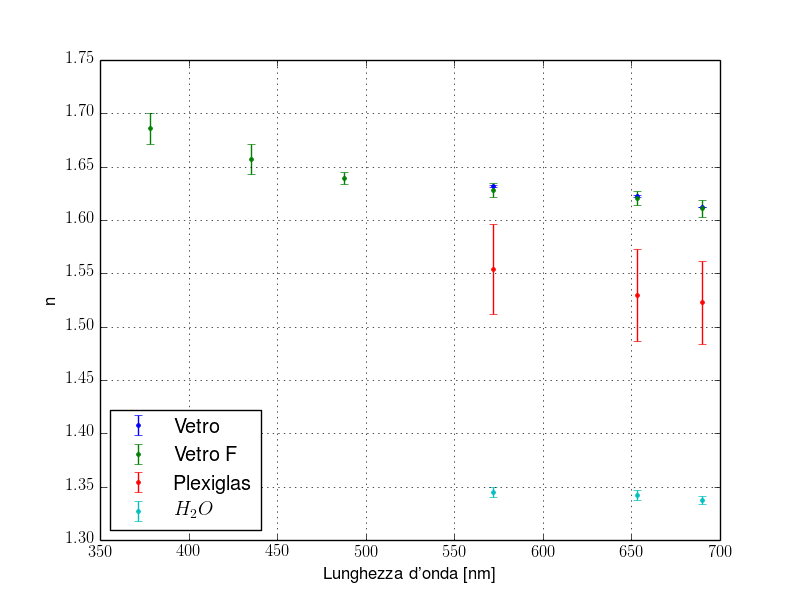
\includegraphics{grafico.png}}
\end{figurehere}
 Per verificare tale dipendenza abbiamo sfruttato la capacità del prisma di scomporre il raggio incidente nelle sue componenti monocromatiche. La dispersione del raggio incidente avviene ad angoli ben precisi nelle condizioni di angolo minimo (come effettuato in laboratorio) e segue la seguente legge.
\begin{equation}
n = \frac{\sin(\frac{\alpha  + \theta}{2})}{\sin(\frac{\alpha}{2})}
\end{equation} 
dove $\alpha$ indica l'angolo di apertura del prisma. \\
Attraverso questa legge è possibile, quindi, associare ad ogni valore di angolo un preciso valore di indice di rifrazione. Tuttavia, per  costruire il grafico in funzione della lunghezza d'onda è necessario sapere a quali valori di $\theta$ è associata ciascuna lunghezza d'onda. Per fare ciò procediamo con il confronto delle nostre misure in ($\theta$, Intensità) e lo spettro dell'elio in ($\lambda$, Intensità). Mettendo a confronto i picchi di intensità è possibile associare ad ogni lunghezza d'onda ad un angolo e con la 
\newline\newline\newline\newline\newline\newline\newline\newline\newline\newline\newline\newline\newline\newline\newline\newline\newline\newline\newline\newline\newline\newline\newline\newline\newline\newline\newline
formula precedente ricavare l'indice di rifrazione $n$.
Per la realizzazione del grafico, sono stati utilizzati gli errori di deviazione standard sugli angoli $\theta$ corrispondenti ai picchi di intensità massima, avendo a disposizione 4 set di dati per ogni materiale, mentre le lunghezze d'onda dell'elio sono state fornite senza errore.\\ 



\end{body}
\end{document}
